\documentclass[10pt,a4paper,conference]{IEEEtran}

% Some very useful LaTeX packages include:
% (uncomment the ones you want to load)

% *** CITATION PACKAGES ***
%
\ifCLASSOPTIONcompsoc
  % IEEE Computer Society needs nocompress option
  % requires cite.sty v4.0 or later (November 2003)
  \usepackage[nocompress]{cite}
\else
  % normal IEEE
  \usepackage{cite}
\fi
% cite.sty was written by Donald Arseneau
% V1.6 and later of IEEEtran pre-defines the format of the cite.sty package
% \cite{} output to follow that of IEEE. Loading the cite package will
% result in citation numbers being automatically sorted and properly
% "compressed/ranged". e.g., [1], [9], [2], [7], [5], [6] without using
% cite.sty will become [1], [2], [5]--[7], [9] using cite.sty. cite.sty's
% \cite will automatically add leading space, if needed. Use cite.sty's
% noadjust option (cite.sty V3.8 and later) if you want to turn this off.
% cite.sty is already installed on most LaTeX systems. Be sure and use
% version 4.0 (2003-05-27) and later if using hyperref.sty. cite.sty does
% not currently provide for hyperlinked citations.
% The latest version can be obtained at:
% http://www.ctan.org/tex-archive/macros/latex/contrib/cite/
% The documentation is contained in the cite.sty file itself.
%
% Note that some packages require special options to format as the Computer
% Society requires. In particular, Computer Society  papers do not use
% compressed citation ranges as is done in typical IEEE papers
% (e.g., [1]-[4]). Instead, they list every citation separately in order
% (e.g., [1], [2], [3], [4]). To get the latter we need to load the cite
% package with the nocompress option which is supported by cite.sty v4.0
% and later. Note also the use of a CLASSOPTION conditional provided by
% IEEEtran.cls V1.7 and later.


% *** GRAPHICS RELATED PACKAGES ***
%
  \usepackage[pdftex]{graphicx}
  \graphicspath{{../Figures/}}
  \DeclareGraphicsExtensions{.pdf,.png}
  \usepackage{color}

% *** MATH PACKAGES ***
%
\usepackage[cmex10]{amsmath}
% A popular package from the American Mathematical Society that provides
% many useful and powerful commands for dealing with mathematics. If using
% it, be sure to load this package with the cmex10 option to ensure that
% only type 1 fonts will utilized at all point sizes. Without this option,
% it is possible that some math symbols, particularly those within
% footnotes, will be rendered in bitmap form which will result in a
% document that can not be IEEE Xplore compliant!
%
% Also, note that the amsmath package sets \interdisplaylinepenalty to 10000
% thus preventing page breaks from occurring within multiline equations. Use:
%\interdisplaylinepenalty=2500
% after loading amsmath to restore such page breaks as IEEEtran.cls normally
% does. amsmath.sty is already installed on most LaTeX systems. The latest
% version and documentation can be obtained at:
% http://www.ctan.org/tex-archive/macros/latex/required/amslatex/math/

%\usepackage{amssymb}%............................ AMS Symbol fonts



% *** SPECIALIZED LIST PACKAGES ***
%
%\usepackage{algorithmic}
% algorithmic.sty was written by Peter Williams and Rogerio Brito.
% This package provides an algorithmic environment for describing algorithms.
% You can use the algorithmic environment in-text or within a figure
% environment to provide for a floating algorithm. Do NOT use the algorithm
% floating environment provided by algorithm.sty (by the same authors) or
% algorithm2e.sty (by Christophe Fiorio) as IEEE does not use dedicated
% algorithm float types and packages that provide these will not provide
% correct IEEE style captions. The latest version and documentation of
% algorithmic.sty can be obtained at:
% http://www.ctan.org/tex-archive/macros/latex/contrib/algorithms/
% There is also a support site at:
% http://algorithms.berlios.de/index.html
% Also of interest may be the (relatively newer and more customizable)
% algorithmicx.sty package by Szasz Janos:
% http://www.ctan.org/tex-archive/macros/latex/contrib/algorithmicx/

% *** ALIGNMENT PACKAGES ***
%
\usepackage{array}
% Frank Mittelbach's and David Carlisle's array.sty patches and improves
% the standard LaTeX2e array and tabular environments to provide better
% appearance and additional user controls. As the default LaTeX2e table
% generation code is lacking to the point of almost being broken with
% respect to the quality of the end results, all users are strongly
% advised to use an enhanced (at the very least that provided by array.sty)
% set of table tools. array.sty is already installed on most systems. The
% latest version and documentation can be obtained at:
% http://www.ctan.org/tex-archive/macros/latex/required/tools/


\usepackage{mdwmath}
\usepackage{mdwtab}
% Also highly recommended is Mark Wooding's extremely powerful MDW tools,
% especially mdwmath.sty and mdwtab.sty which are used to format equations
% and tables, respectively. The MDWtools set is already installed on most
% LaTeX systems. The lastest version and documentation is available at:
% http://www.ctan.org/tex-archive/macros/latex/contrib/mdwtools/

% IEEEtran contains the IEEEeqnarray family of commands that can be used to
% generate multiline equations as well as matrices, tables, etc., of high
% quality.

% *** SUBFIGURE PACKAGES ***
\ifCLASSOPTIONcompsoc
  \usepackage[caption=false,font=normalsize,labelfont=sf,textfont=sf]{subfig}
\else
  \usepackage[caption=false,font=footnotesize]{subfig}
\fi

%Setting captions to centered (Not IEEE journal standard)
%\makeatletter
%\long\def\@makecaption#1#2{\ifx\@captype\@IEEEtablestring%
%\footnotesize\begin{center}{\normalfont\footnotesize #1}\\
%{\normalfont\footnotesize\scshape #2}\end{center}%
%\@IEEEtablecaptionsepspace
%\else
%\@IEEEfigurecaptionsepspace
%\setbox\@tempboxa\hbox{\normalfont\footnotesize {#1.}~~ #2}%
%\ifdim \wd\@tempboxa >\hsize%
%\setbox\@tempboxa\hbox{\normalfont\footnotesize {#1.}~~ }%
%\parbox[t]{\hsize}{\normalfont\footnotesize \noindent\unhbox\@tempboxa#2}%
%\else
%\hbox to\hsize{\normalfont\footnotesize\hfil\box\@tempboxa\hfil}\fi\fi}
%\makeatother


% *** FLOAT PACKAGES ***
%
\usepackage{fixltx2e}
% fixltx2e, the successor to the earlier fix2col.sty, was written by
% Frank Mittelbach and David Carlisle. This package corrects a few problems
% in the LaTeX2e kernel, the most notable of which is that in current
% LaTeX2e releases, the ordering of single and double column floats is not
% guaranteed to be preserved. Thus, an unpatched LaTeX2e can allow a
% single column figure to be placed prior to an earlier double column
% figure. The latest version and documentation can be found at:
% http://www.ctan.org/tex-archive/macros/latex/base/

% *** PDF, URL AND HYPERLINK PACKAGES ***
%
\usepackage{url}

\usepackage{sistyle}
    \SIstyle{S-Africa}
    \SIunitspace{{\cdot}}
    \SIunitdot{{\cdot}}

% generate nice bookmarks and hyperrefs when exporting to pdf and dvi (screen version):
\usepackage[a4paper,plainpages=false,colorlinks,linktocpage,bookmarks=true,bookmarksopen=false]{hyperref}
% use this for printing only (no color, print version):
%\usepackage[a4paper,plainpages=false,colorlinks=false,linktocpage,bookmarks=true,bookmarksopen=false]{hyperref}

% correct bad hyphenation here
\hyphenation{op-tical net-works semi-conduc-tor}

%Add elegant support for Big-O notation
\providecommand{\OO}[1]{\operatorname{O}\left(#1\right)}

\begin{document}

%
% paper title
\title{Pithos: A Hybrid Multi-Tiered State Persistency Architecture for Peer-to-Peer Massively Multiuser Virtual Environments}

%\author{\IEEEauthorblockN{John S. Gilmore and Herman A. Engelbrecht\\}
%\IEEEauthorblockA{MIH Media Lab\\
%Electronic Engineering Department\\
%Stellenbosch University\\
%Stellenbosch, South Africa\\
%mail: jgilmore@ml.sun.ac.za and hebrecht@sun.ac.za}}

\maketitle

\begin{abstract}
%\boldmath
The abstract goes here

\end{abstract}


\section{Introduction}
\label{introduction}

%
% Admittedly, this is a hack and may well be fragile, but seems to do the
% trick for me. Note the need to keep any \label that may be used right
% after \section in the above as the hack puts \section within a raised box.

% The very first letter is a 2 line initial drop letter followed
% by the rest of the first word in caps (small caps for compsoc).
%
% form to use if the first word consists of a single letter:
% \IEEEPARstart{A}{demo} file is ....
%
% form to use if you need the single drop letter followed by
% normal text (unknown if ever used by IEEE):
% \IEEEPARstart{A}{}demo file is ....
%
% Some journals put the first two words in caps:
% \IEEEPARstart{T}{his demo} file is ....
%

%P2P MMVE Background
\IEEEPARstart{P}{eer-to-Peer (P2P)} Massively Multiuser Virtual Environments (MMVEs) have received significant attention from the research community,
since the first publication on the subject by Knutssonn et al. in 2004 \cite{knutsson_p2p_first}. P2P MMVEs promise to solve many issues prevalent in
today's Client/Server (C/S) based MMVEs. Some key issues have to be solved before P2P MMVEs can be implemented commercially. Over the past few years,
researchers have been addressing these challenges.

%Key challenges and focus
Recently, six key challenges of P2P systems have been identified: Interest Management, Game Event Dissemination, Non-player Character (NPC) Host
Allocation, Game State Persistency, Cheating Mitigation and Incentive Mechanisms \cite{Fan_deisgn_issues_p2p}. Most of the challenges mentioned have
received significant attention from the research community, except for state persistency.

State persistency defines how object states should be stored. This allows for storing anything from a user's position to the state of the virtual
market in an MMVE. For a P2P MMVE, game data must be distributed amongst various peers in the network. This creates challenges not usually present in
classic C/S MMVEs. The focus of this paper is exclusively on state persistency in P2P MMVEs.

%Current techniques not perfect
The paper first attempts to group state persistency mechanisms found in the literature. The paper then shows that none of the approaches to state
persistency has thus far been sufficient to meet the storage requirements of MMVEs of today. All storage models are evaluated according to the
identified requirements of scalability, fairness, reliability, responsiveness and security.

%Propose multi-tiered model
Because current state persistency models do not address all the requirements of modern MMVEs, a novel hybrid multi-tiered state persistency model is
proposed, called Pithos, that is based on grouping players in some logical way and allowing for responsive interaction between players in the same
group, with lower levels of responsiveness between groups. The supposition is that players have more interest in other object and player states close
to them than far from them.

%Implementation
The proposed multi-tiered model is currently being implemented in Oversim, a peer-to-peer simulation environment based in Omnet++. The model allows
for the measurement of the requirements of scalability, fairness, reliability and responsiveness. Furthermore, it allows for the comparison of the
current model with other state persistency models. Initial results seem promising, with the implemented model functioning as expected. The system
shows to be very responsive when storing data within a group and as responsive as storing data in an overlay when storing data between groups.

%Summary
Section \ref{current_models} groups storage models found in the literature and describes the advantages and disadvantages of each group. The section
concludes with a comparison of the different storage models and comments on their applicability to P2P MMVEs.
%
Section \ref{proposed_model} introduces our proposed state persistency model and describes the different assumptions on which it is based.
%
Section \ref{implementation} describes the implementation details of the proposed model.
%
Section \ref{results} presents some preliminary results.
%
Section \ref{conclusion} concludes with a summary of the paper and a discussion on possible future work.

\section{Current state persistency models}
\label{current_models}

%Overview of four approaches
Four approaches have been identified by which state persistency is achieved in P2P MMVEs. These are: \emph{super peer storage}, \emph{overlay
storage}, \emph{distance-based storage} and \emph{hybrid storage}. Requirements have also been identified by which storage systems should be
measured. These are: scalability, fairness, reliability, responsiveness and security.

%Scalability
For an MMVE state persistency architecture to be scalable, it should be able to support large, typically thousands of users. In the paper,
scalability it not handled as some separate entity, but rather all other requirements are evaluated in terms of a system of thousands of users.
%Reliability
Reliability is defined to mean that a file in the storage system may neither be lost, nor not be available when a user requests it.
%Fairness
For a system to be fair, the responsibility of storage should be equally shared amongst all users. Ideally, a fair scheme should take the
heterogeneity of peers into account. This ensures that costs due to bandwidth and storage are shared amongst all users.
%Responsiveness
Responsiveness is a requirement that has not really been part of file storage systems in the past. Usually, it doesn't matter much how low it takes
to resolve a file storage or request, just that the file is stored or retrieved. Sizes of files are usually large and so the time storage and
retrieval operations take are usually constrained by the available bandwidth. For games, it is believed that responsive object storage is a key
requirement to promote responsive gameplay and robust recovery mechanisms. Especially because it is expected that game objects are in general much
smaller than the files, which normal storage systems are designed for.
%Security
Data security is a major issue for distributed storage, because data are stored on users' machines who should not necessarily be able to access and
alter the data stored.

To clarify what type of objects are stored in these types, only the root objects, also called the authoritive objects, are considered for storage. It
is still assumed that replica objects that are used by players to render the world are locally stored and that these objects derive their states from
the respective root objects.

\begin{table*}[htbp]
\centering
\begin{tabular}{|r|c|c|c|c|}
\hline
Storage type & Reliability & Responsiveness & Security & Fairness\\
\hline
Super Peer & Medium & High & Low & Low\\
Overlay & High & Low & Medium & High\\
Hybrid & High & High & Medium & Low\\
Distance-based & Medium & High & Low & Medium\\
\hline
\end{tabular}
\caption{Differences between storage mechanisms} \label{tab_storage}
\end{table*}
%
Table \ref{tab_storage} presents a characterisation of current storage systems according to the characteristics defined. Table \ref{tab_storage} also
provides some references that act as examples of the different storage types mentioned. These example architectures will be discussed briefly in the
sections to follow.

\subsection{Super peer storage}

%Super peer storage - description
Super peer storage relies on the super peer storing all information that is in its domain \cite{knutsson_p2p_first}. A domain is usually created by
segmenting the world into regions and super peers act as regional servers to all peers in their region. Each super peer handles state persistency for
its region, hosting NPCs, objects and persistent player data. This storage method is much like a Client/Server setup, with the super peer acting as
the server for the virtual geographic region assigned to it.

The advantage of super peer storage is that it's fairly simple to implement using well known database solutions.

The disadvantages of super peer storage stem from the per-region centralised approach. It is difficult to achieve high levels of reliability, without
some migration mechanism that requires redundant super peers per region and allows for migration of data and responsibilities when a super peer
leaves the network. Because super peers are merely users in the virtual world, they can be expected to regularly join and leave the world. It is
possible to implement such mechanisms, although that would significantly complicate the implementation task. No current architectures are known to
have implemented such a mechanism so the difficulties associated with this approach have not been explored.

The main issues with super peer storage are those of fairness and security. Because a single super peer controls all data in a region and because
that super peer is merely another user, there might be a high possibility that the data can be compromised in some way. There is also a high
incentive to be able to modify data in a region by a user operating in that region. It is also difficult to secure the data, because any user should
have access to, for example, another user's position. If the super peer user can identify which data is which, he might be able to modify that data.

Fairness is another issue with super peer storage, because the super peers are expected to store all the region data and are also expected to donate
their bandwidth to service requests for data from all region peers.


\subsection{Overlay storage}

%Description
Overlay storage is classified as using any type of structured P2P overlay to store data in a distributed fashion \cite{Douglas05enablingmassively},
\cite{using_freenet_storage}, \cite{Fan_phd}, \cite{past_storage_focus}. This is a very broad definition, which basically encompasses any P2P
distributed storage currently in use. Some examples and a comparison of different distributed storage techniques can be found in
\cite{Hasan_distributed_storage_survey}. The reasoning is that any P2P distributed storage can be used to only store game files. Therefore,
distributed storage is used as a distributed database for game files.

%Advantages/Disadvantages
The main advantages of overlay storage is its reliability and fairness. Because data are distributed across all nodes, overlay storage is the fairest
storage system reviewed. Because data are hosted by many nodes, redundancy may be used to make the system reliable. Because of the distance based
routing mechanism used in most P2P overlays, redundancy is easily implemented by placing replica data at a node's overlay neighbours. Overlay storage
can also be made reasonably secure, because it is possible to leverage the redundancy mentioned and multiple routing paths present in the overlay.

The main disadvantage of overlay storage is responsiveness. The routing time in overlay storage is of order $O(\log(N))$, where N is the total number
of nodes in the network. This can be considered an efficient routing time in general, but for real-time applications that require real-time access to
data, this routing complexity is not considered ideal.

\subsection{Hybrid storage}

%Description
The world is divided into regions, with each region controlled by a super peer \cite{zoned_federation}, \cite{hybrid_storage1}. The complete region
state is cached at every super peer, the same as with super peer storage. There also exists a backup overlay storage architecture, to which data may
be backed up for long term, redundant and secure storage. The hybrid region-based overlay storage contains many improvements over pure overlay
storage as will be discussed in the following sections.

%Advantages/Disadvantages
Hybrid storage combines some of the features present in overlay and super peer storage to have the advantages of high reliability and responsiveness.
Reliability is achieved from redundancy present in overlay storage and responsiveness is achieved by the direct access peers have to their respective
super peer.

Hybrid storage still partly suffers from the security issues present in super peer storage, but overlay storage allows for replication which creates
reference objects to which the super peer objects might be compared. Checking every super peer object against the corresponding overlay object will,
however negate any advantages received from super peer storage in terms of responsiveness.

Hybrid storage still suffers from the lack of fairness present in super peer storage. Although data are distributed amongst all nodes for overlay
storage, there still exists super peer nodes that also possess all data present in the network, making the storage almost as unfair as super peer
storage.

\subsection{Distance-based storage}

%Description
Distance based approaches, such as the Voronoi storage approaches \cite{Buyukkaya_voronoi_state_management}, \cite{Hu_voronoi_IM} and some more
general approaches \cite{colyseus_distance_based}, \cite{solipsis}, store object data on the peer closest to the object in the virtual world. Some
distance metric is used to determine on which node an object should be stored. In some systems, only player states are considered for storage
\cite{individual_storage1}, \cite{cheat_proof_playout}. This storage is termed individual storage and is considered as a subset of distance storage,
which also allows for non-player objects to be stored.

%Advantages/Disadvantages
Responsiveness is considered to be the main advantage of distance-based storage. It is considered that the player that is close to an object has more
interest in that object than a player that is far away. This means that the player with the most interest in an object will be most likely to be
locally hosting that object. This is not always the case, but for cases where the player hosting the object has to serve that object to another
player, the system is still as responsive as super peer and normal C/S-based storage. Distance-based storage can also be made reliable by
implementing some replication and migration mechanisms or implementing it as a distance-based overlay storage hybrid. Such implementation have not
been presented in the literature reviewed.

Two issues with distance-based storage are security, and to a lesser degree, fairness. Security is a major concern, since data are by design, stored
on nodes with the most interest in it. This means that a node that stores data has the most interest to be able to modify that data in contravention
of the virtual environment rules. Although all nodes share all objects in the virtual world, some nodes might have to store more data than others
depending on user density in the virtual world and on how many objects are close to the different nodes.

\subsection{Centralised storage}

%Description
Some P2P MMVEs use centralised storage, where all peers store data in a centralised database \cite{badumna_engine},
\cite{rooney_centralised_storage}, \cite{hybrid_p2p_cs_centralised}.

%Advantages/Disadvantages
This type of storage suffers from all the scalability and single point of failure issues present in a centralised system. Consequently, most of the
advantages of P2P MMVEs are forgone by this type of storage. When compared to the requirements mentioned in Section \ref{current_models}, centralised
storage suffers from fairness and reliability issues.

\subsection{Summary and comparison}

From this discussion, it is evident that none of the mentioned storage types in their current forms are appropriate for data storage in MMVEs. None
of the storage types meet all the requirements as set out. Super peer storage is not fair or secure, overlay storage is not responsive, hybrid
overlay/super peer storage is not fair and distance-based storage is not secure and not yet reliable.

It should also be noted that most of these storage types are not mature. In the referenced papers, they were mentioned as a means by which
persistency might be achieved. But none of the papers presented concrete design, implementation and results on the performance of the storage types,
except for the PAST implementation, which is an overlay storage type.

This shows that not only is a storage type required that improves upon past storage types, but a concrete design and implementation is also required
that would lay bare any unforeseen issues that might arise when implementing P2P MMVEs. The following sections attempt to provide such a design and
such an implementation.

While the system is not yet complete, some promising preliminary results are also shown. These results show the improvements in terms of
responsiveness and fairness achieved.

\section{Pithos: the proposed state persistency architecture}
\label{proposed_model}

In this section ``Pithos'', the proposed P2P MMVE state persistency architecture is described. The architecture uses hybrid techniques, grouping and
multiple tiers to improve upon current storage systems.

The inspiration for this architecture came from two observations. Firstly: one can combine multiple storage models and arrive at a model which
possesses fewer disadvantages than any of the models used. It is supposed that one might arrive at a model which possesses none of the disadvantages
of any of the models used, if the models are carefully chosen.

Secondly, responsiveness is greatly increased in a fully distributed model, where there is no intermediate server that relays all information. It
was, however, also observed that fully distributed architectures are not scalable because of the number of messages scaling by an $O(N^2)$, where $N$
is the number of nodes in the network.

\subsection{Architecture}

\begin{figure}[htbp]
 \centering
 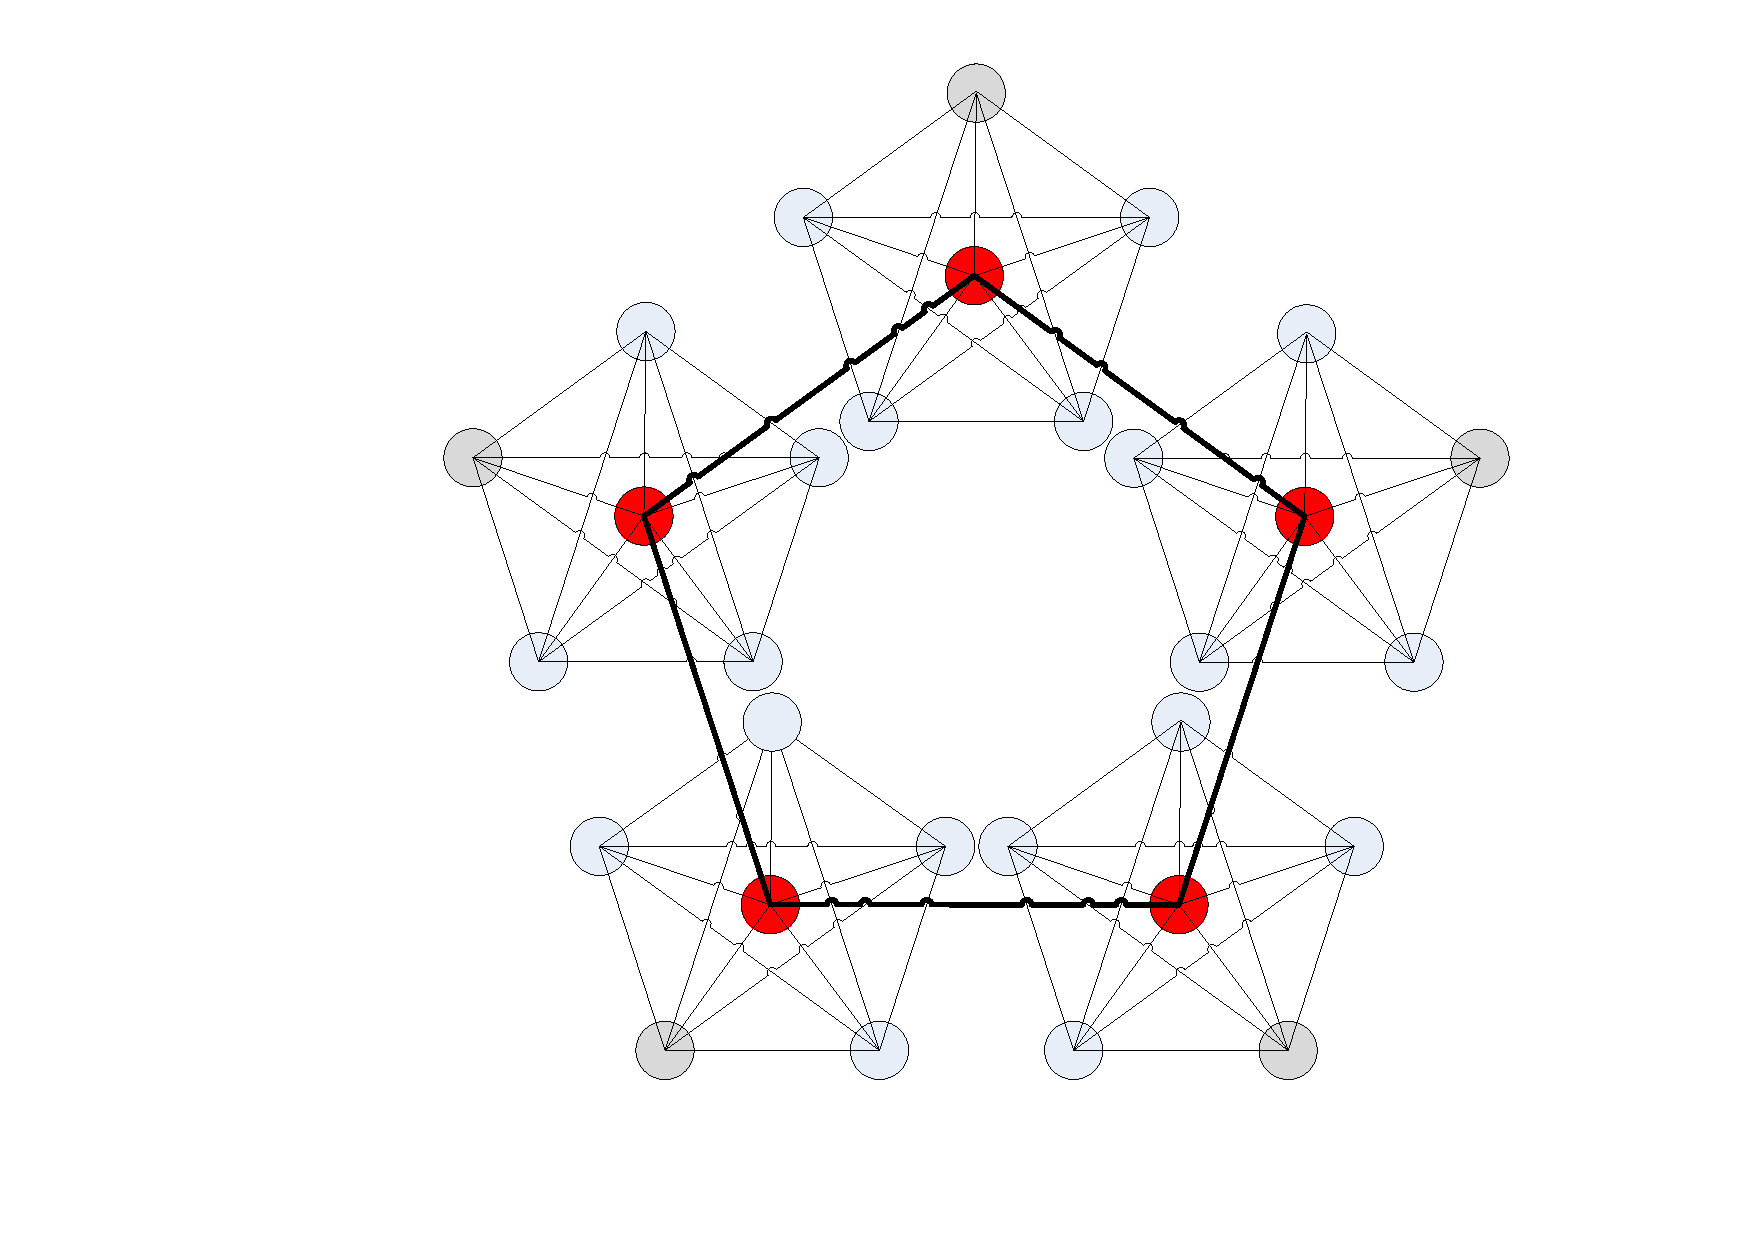
\includegraphics[clip=true, viewport=7.5cm 2.5cm 26cm 20cm, width=0.7\columnwidth]{CDHT_layout}
 \caption{Layout of the Pithos storage architecture}
 \label{fig_pithos}
\end{figure}
%
Figure \ref{fig_pithos} shows the Pithos architecture. The figure shows groups of fully connected peers (blue and red), where all groups are
connected to each other in an P2P overlay through super peers (red). This section described the general architecture of Pithos, the following
sections then describe how each of the requirements of fairness, reliability, responsiveness and security are achieved in Pithos.

Pithos groups peers in some way to form a two tiered storage model. The first tier is a storage model at group level and the second is a model over
all groups. On the first tier, which is the intra group level, a fully distributed storage system is used to allow for highly responsive read and
write operations within the group. On the second tier, which is the inter group level, overlay routing is used to store data between groups.

\subsubsection{Grouping}

%Speak more concretely of grouping algorithms
At the core of the architecture is how peers are grouped. Two approaches are being evaluated to group peers, one is by using distributed clustering
techniques, for example affinity propagation \cite{affinity_propagation}, the other is by using dynamic regioning techniques, for example spatial
publish subscribe.

One method by which peers might be grouped is merely to use peer proximity and movement and thereby define groups as groups of users in the virtual
world. The architecture will then make use of the flocking behaviour of players to dynamically group players into flocks or clusters \cite{flocking}.
The main idea of flocking is that players move around in groups, rather than randomly on their own. Because of the flocking behaviour of players,
dynamic groups or regions that move with groups of players may be a better fit than static or even dynamic regions that operate on areas of the
virtual world and not on how groups of players actually cluster.

Because a fully distributed architecture is not scalable, group sizes should also not exceed some threshold. This threshold complicates group
construction, because groups are already constructed according to position in the virtual world.

As an alternative to geographic grouping, dynamic regioning might also be used to group players. Where every dynamic region will constitute a group
of players. Dynamic regioning splits an overpopulated region which will allow for sufficient bounding of the amount of players in the group.

%Speak about Spatial Publish Subscribe

\subsubsection{Joining}

When a Super Peer is created, it registers its IP address and position within the virtual world with the Directory Server. When a peer joins the
network it sends its position to the directory server and receives a super peer IP that is closest in return. The peer then sends a join request to
the received super peer IP. The super peer can accept the request or reply with another super peer IP that it deems more appropriate. The super peer
also sends a list of all peer IPs that are currently part of the group to the joining peer. In addition, the super peer updates its group peers with
the IP of the joining node.

Here it is possible to use a simple underlay network, where nodes are positioned on Euclidean space and latencies are calculated according to the
distances between nodes or to use a modified version of the INET framework found in Omnet++, which attempts to accurately model latency effects and
the various complexities of the underlying network.

\subsubsection{Store and retrieve with replication}

Pithos implements data replication to enable it to handle node churn. If a node leaves the network and stops to transmit pong messages, the migration
mechanism will detect this and replicate the file on another node. Replication exists intra as well as inter group.

\subsubsection{Secure node ID assignments}

\subsection{Responsiveness}

If players are grouped more intelligently, less traffic will have to flow between groups, which will reduce the number of queries to the DHT, which
in turn will improve the latency of the overall system. Using groups or flocks would, therefore, compliment this technique.

%\subsection{Distance-based}
\label{distance_based}

%Why distance based and grouping might help for saving game data

\subsection{Reliability}

%\subsection{Bootstrap mechanism}

\subsection{Fairness}


\subsection{Security}

%\subsection{Certification Authority}

Use secure node ID assignments, by making use of a Certification Authority, or designing the system in such a way that a peer cannot select or report
it's own node ID.

\subsection{Future work}

The issue with such a system would be how to uniquely identify a group and how the identification would be applied when groups merge or split. Groups
moving towards each other also have to be identified and the grouping might have to be able to maintain two groups moving through each other. Little
work has been done to group players in a distributed fashion in virtual worlds. Further research is required into grouping algorithms to determine
their usability in virtual worlds under user churn.

\subsection{Future work}

The simulation does not yet support nodes leaving the network. The migration mechanism should still be implemented before rigourous testing under
heavy network churn will become a possibility.

%Don't send complete files

%Use KBRTestApp

\section{Preliminary results}
\label{results}

For preliminary results, two requirements were measured. These were responsiveness and fairness. Responsiveness is defined as how long it takes to
store and retrieve a node from the network. Fairness is defined as the variance in the number of files or bytes stored on the different nodes.

The responsiveness is compared to Pastry routing times.

\subsection{Test setup}
In the results shown, Pastry was used as an overlay, Pithos as the tier 1 application and another ``game'' application was used as the tier 2
application. The purpose of the game application is to drive the simulation with put and get requests. Pastry was chosen because of many articles
referencing Pastry as the overlay used for overlay storage. It is important to note that because of Oversim's layered architecture, Pithos can work
and has been additionally tested with Chord and Kademlia. The ideal choice of overlay is a question for future research and testing.

In the tier 1 layer, a specific number of peers, super peers and a single directory server is created at the start of the simulation. Every node is
allowed to fully initialise before it starts to generate and respond to store and retrieve requests. For the results shown in Section \ref{results},
14999 peer, 499 super peers and 1 directory server were used to give a total of 15000 simulated nodes. This limit is established by the number of
node coordinates in the Oversim coordinates file.

After a specific node has joined a group, it informs the game module and the game module then starts to generate store and retrieve requests. These
requests are received by the tier 1 peer logic module and handled.

\subsection{Responsiveness}

Firstly, we evaluate the responsiveness of the storage system. In the storage system, we expect two levels of responsiveness. We expect a certain
level of responsiveness for intra group communications and a certain level of responsiveness for inter group communications. Because we expect intra
group communications to appear more often, we can calculate an average response time which is determined by the percentage of intra group requests,
compared to inter group requests.

\begin{figure}[htbp]
 \centering
 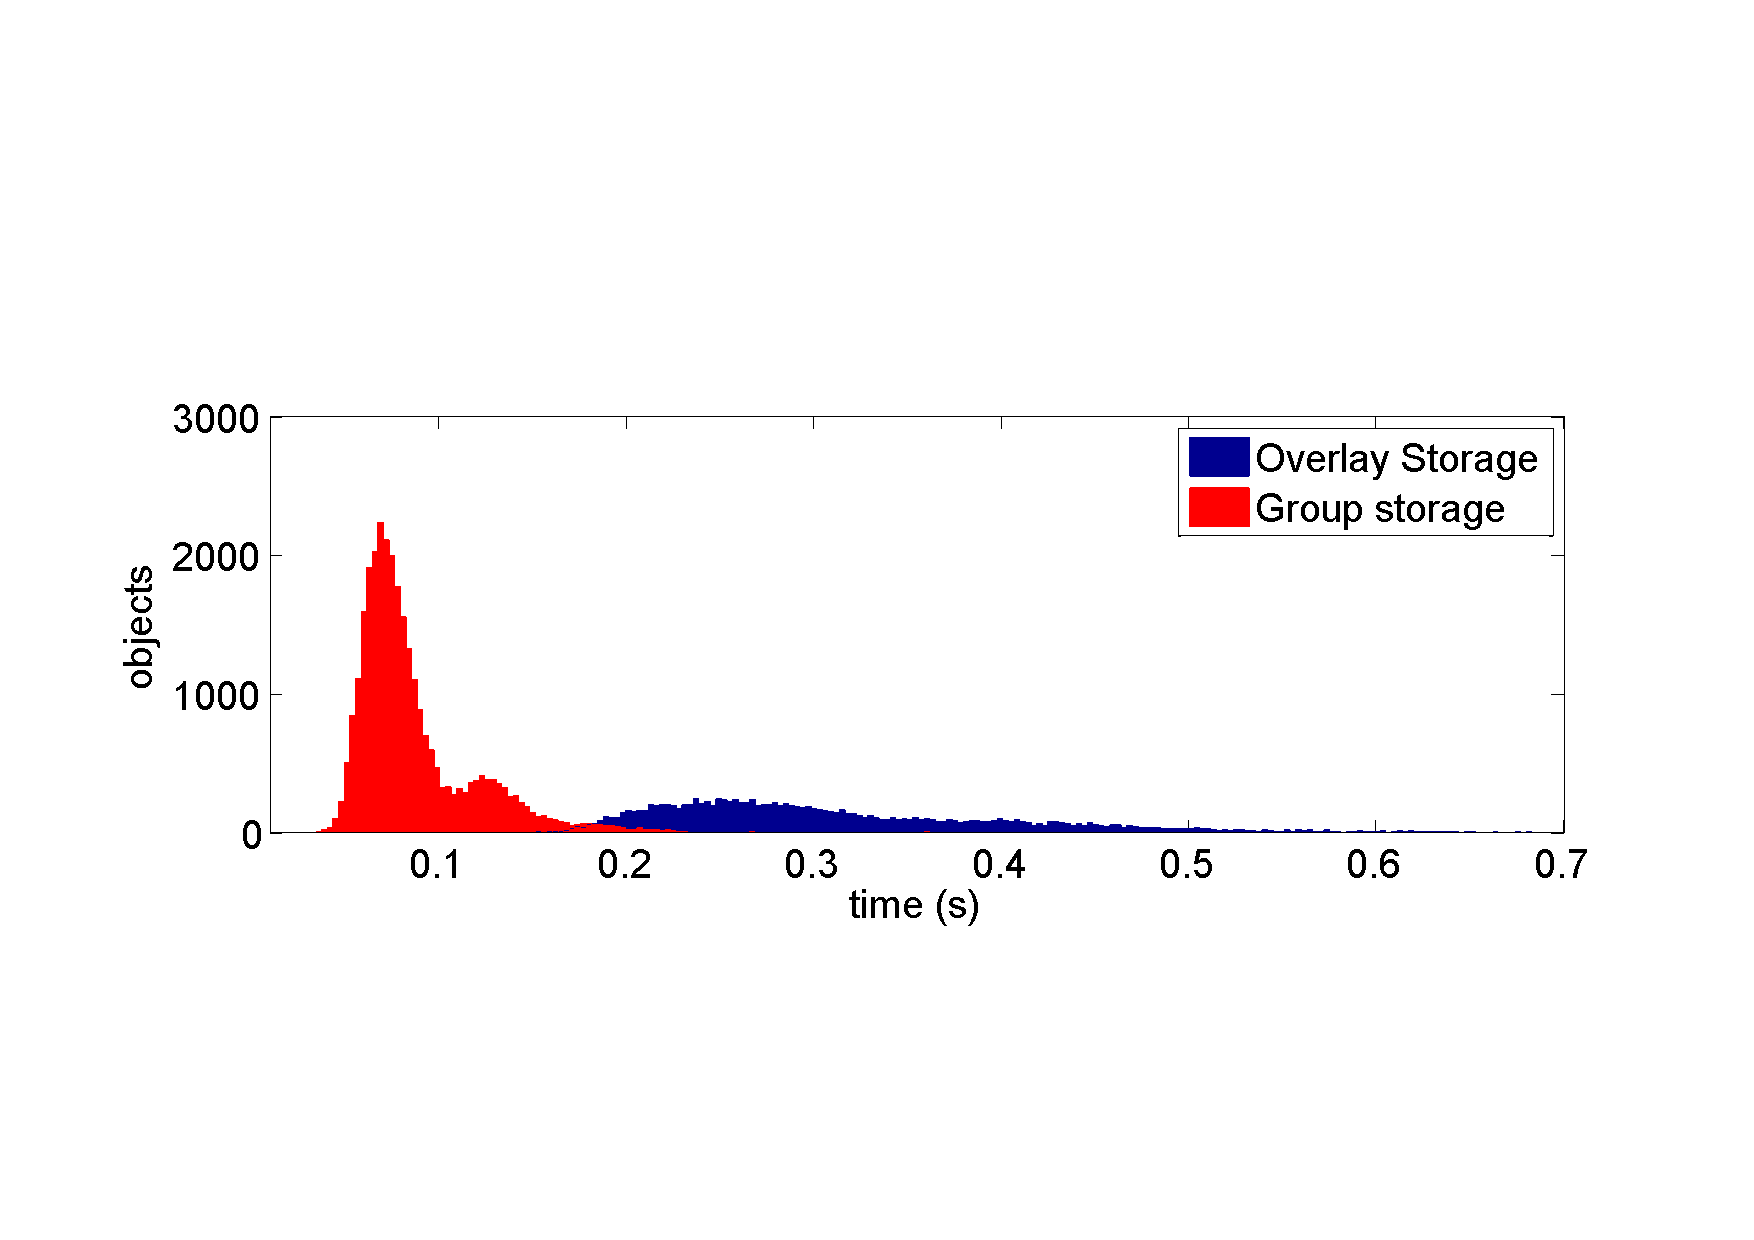
\includegraphics[clip=true, viewport=1.5cm 1.3cm 25.5cm 19.7cm, width=\columnwidth]{request_time_distribution}
 \caption{Time distribution of overlay and root/replica objects}
 \label{fig_pithos_response}
\end{figure}
%
Figure \ref{fig_pithos_response} shows the distribution of mean storage request times over all nodes in the network for the different types of
storage present in the network. One can see that the intra group root and replica objects are stored much faster than the overlay objects in the
network. Specifically, intra group object are stored in a mean time of 0.0878 s, while inter group objects are stored in a mean time of 0.3284 s,
3.74 times slower than intra group stores.

There seem to be multiple distributions of root and replica nodes spaced equally apart. The supposition is that these represent the physical hops in
the underlaying architecture.

From Figure \ref{fig_pithos_response} it is evident that if only overlay storage is used, the storage and retrieval times will be much higher.

To exactly compare Pithos with overlay storage, the percentage of intra group requests compared to inter group requests should first be known.
%Insert other Matlab responsiveness calculations

\begin{figure}[htbp]
 \centering
 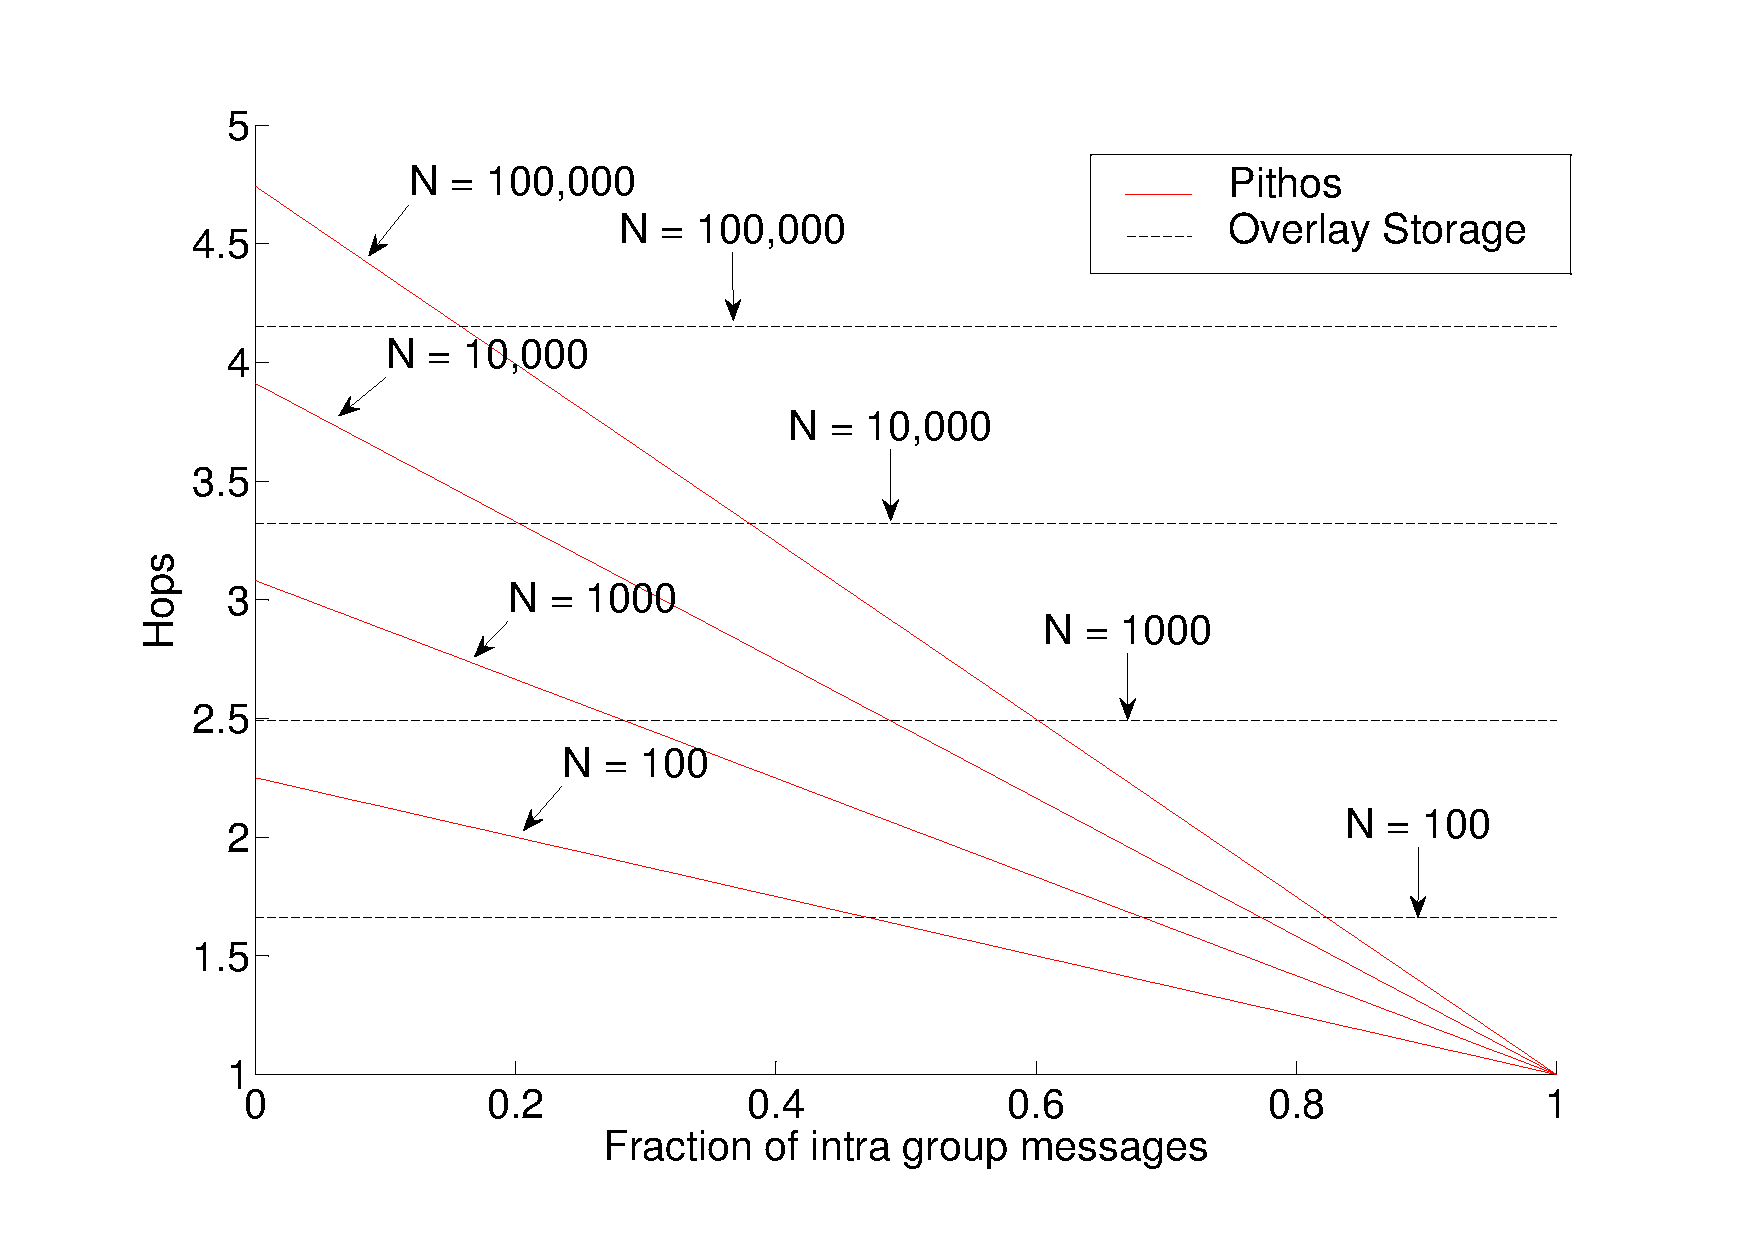
\includegraphics[clip=true, viewport=2cm 1cm 27cm 19.5cm, width=\columnwidth]{Hops_vsGroupFrac_4n}
 \caption{Time distribution of overlay and root/replica objects}
 \label{fig_pithos_response}
\end{figure}


\subsection{Fairness}

\begin{figure}[htbp]
 \centering
 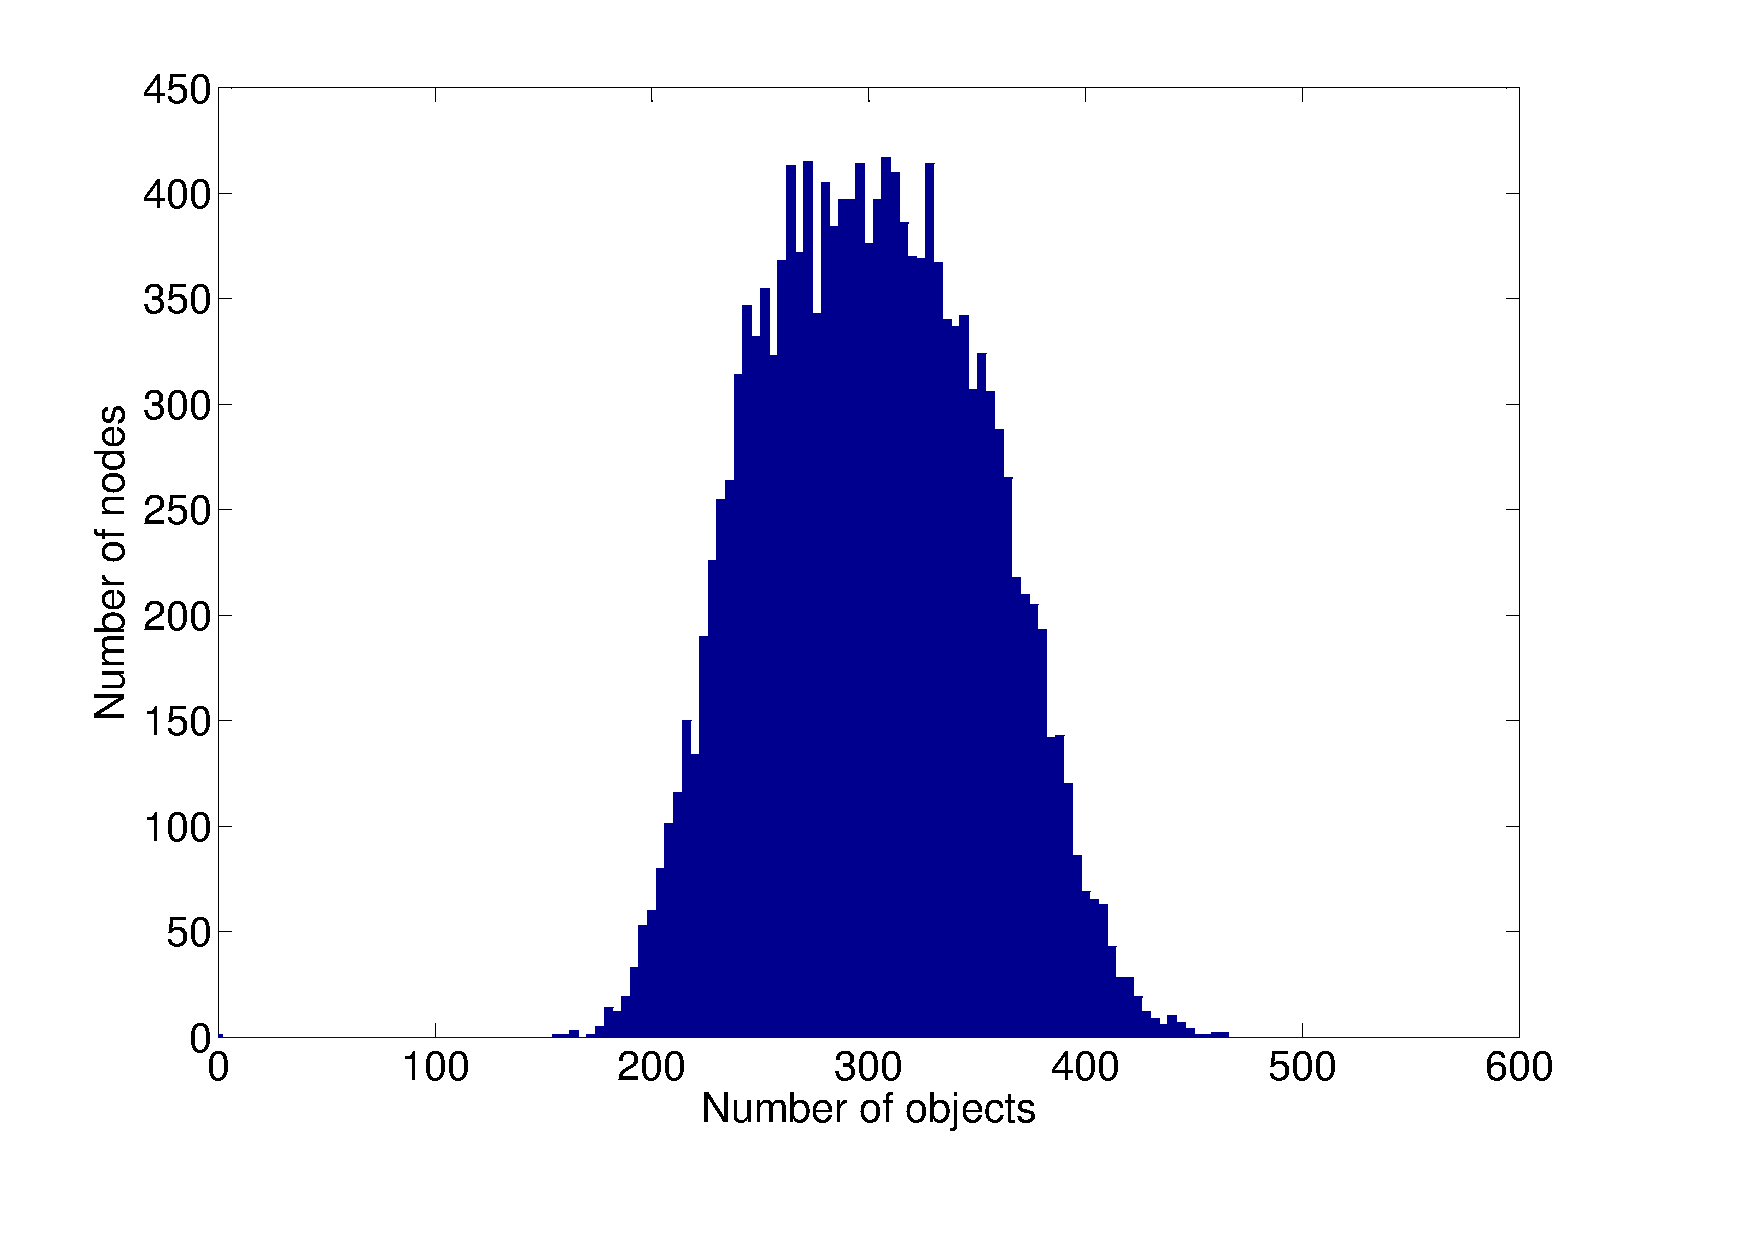
\includegraphics[clip=true, viewport=1.5cm 1.8cm 26.5cm 20cm, width=\columnwidth]{RootRepObjects}
 \caption{Root/Replica object number distribution}
 \label{fig_pithos_response}
\end{figure}

\begin{figure}[htbp]
 \centering
 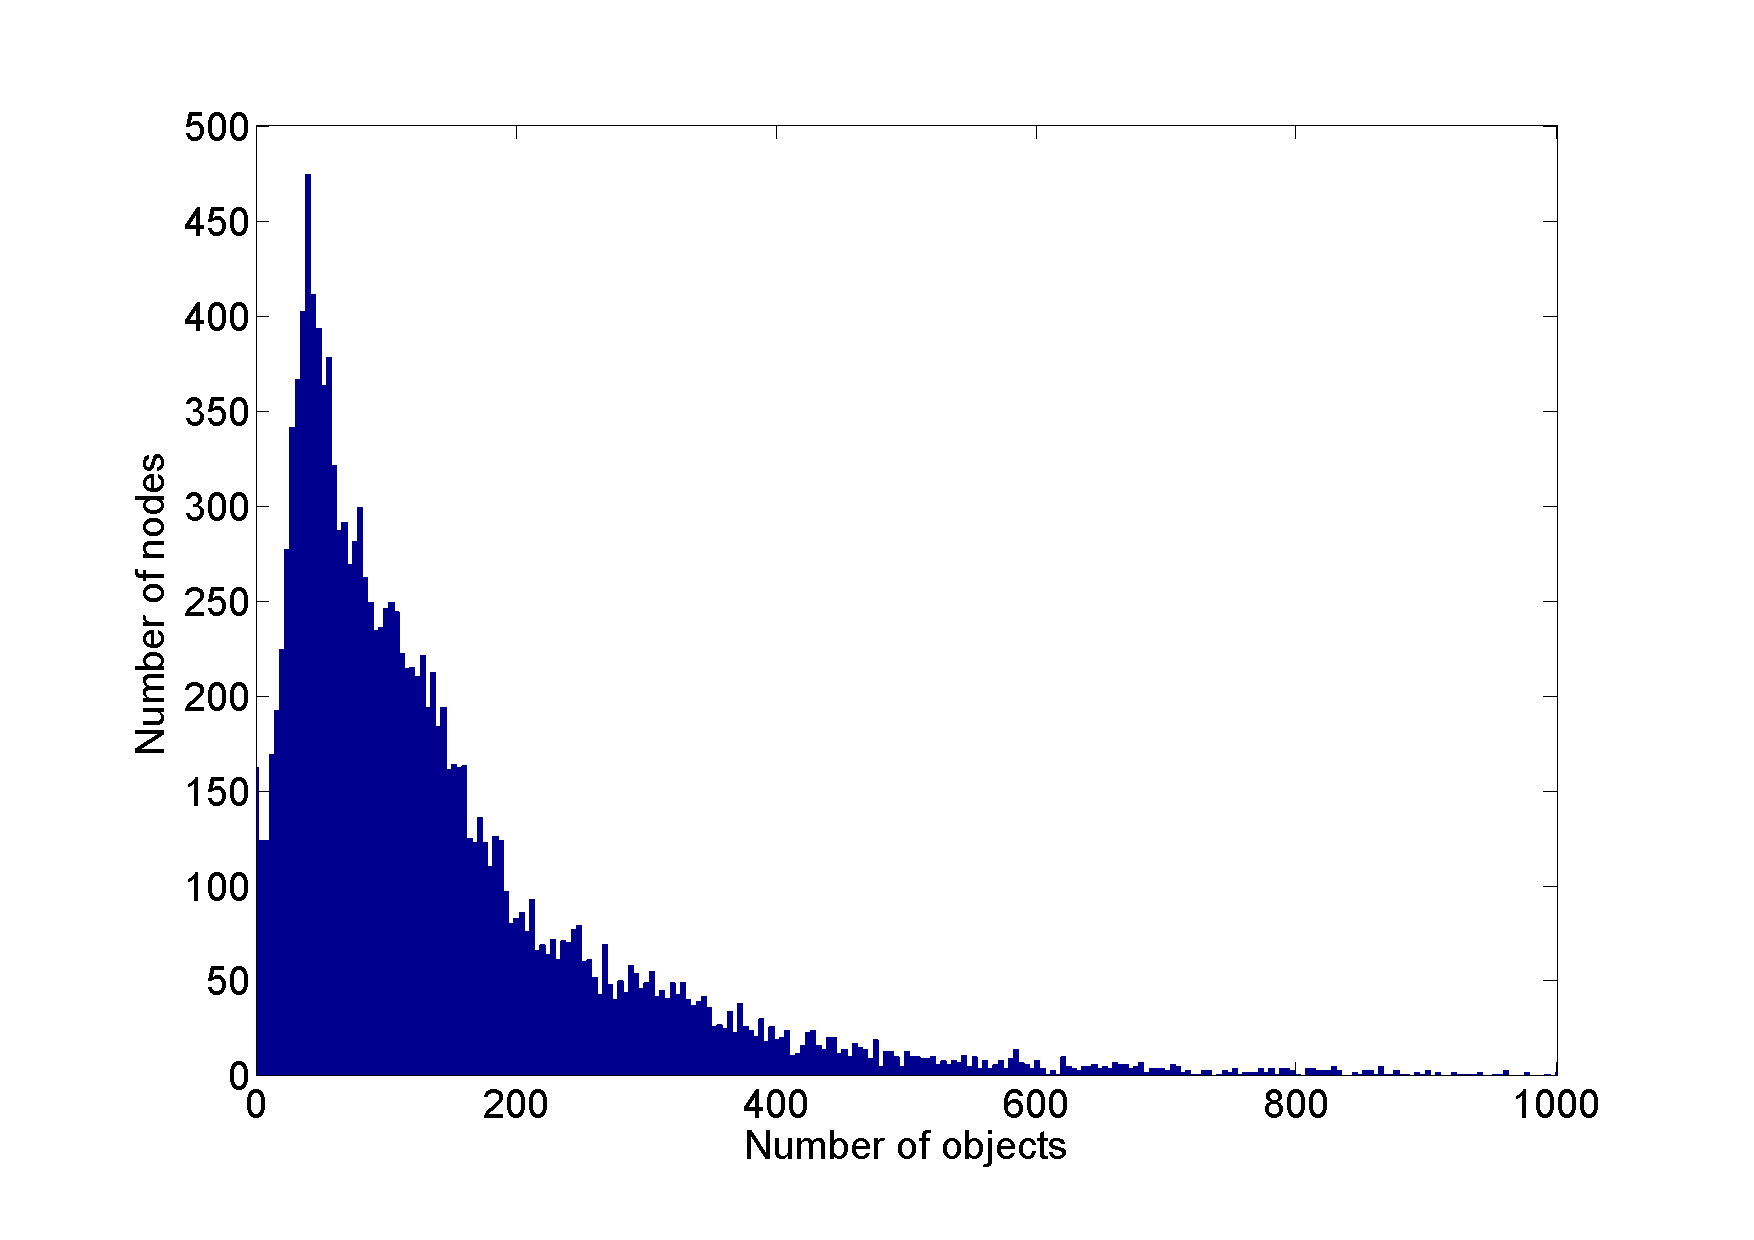
\includegraphics[clip=true, viewport=1.5cm 1.2cm 27cm 19.7cm, width=\columnwidth]{OverlayObjects}
 \caption{Overlay object number distribution}
 \label{fig_pithos_response}
\end{figure}

\begin{figure}[htbp]
 \centering
 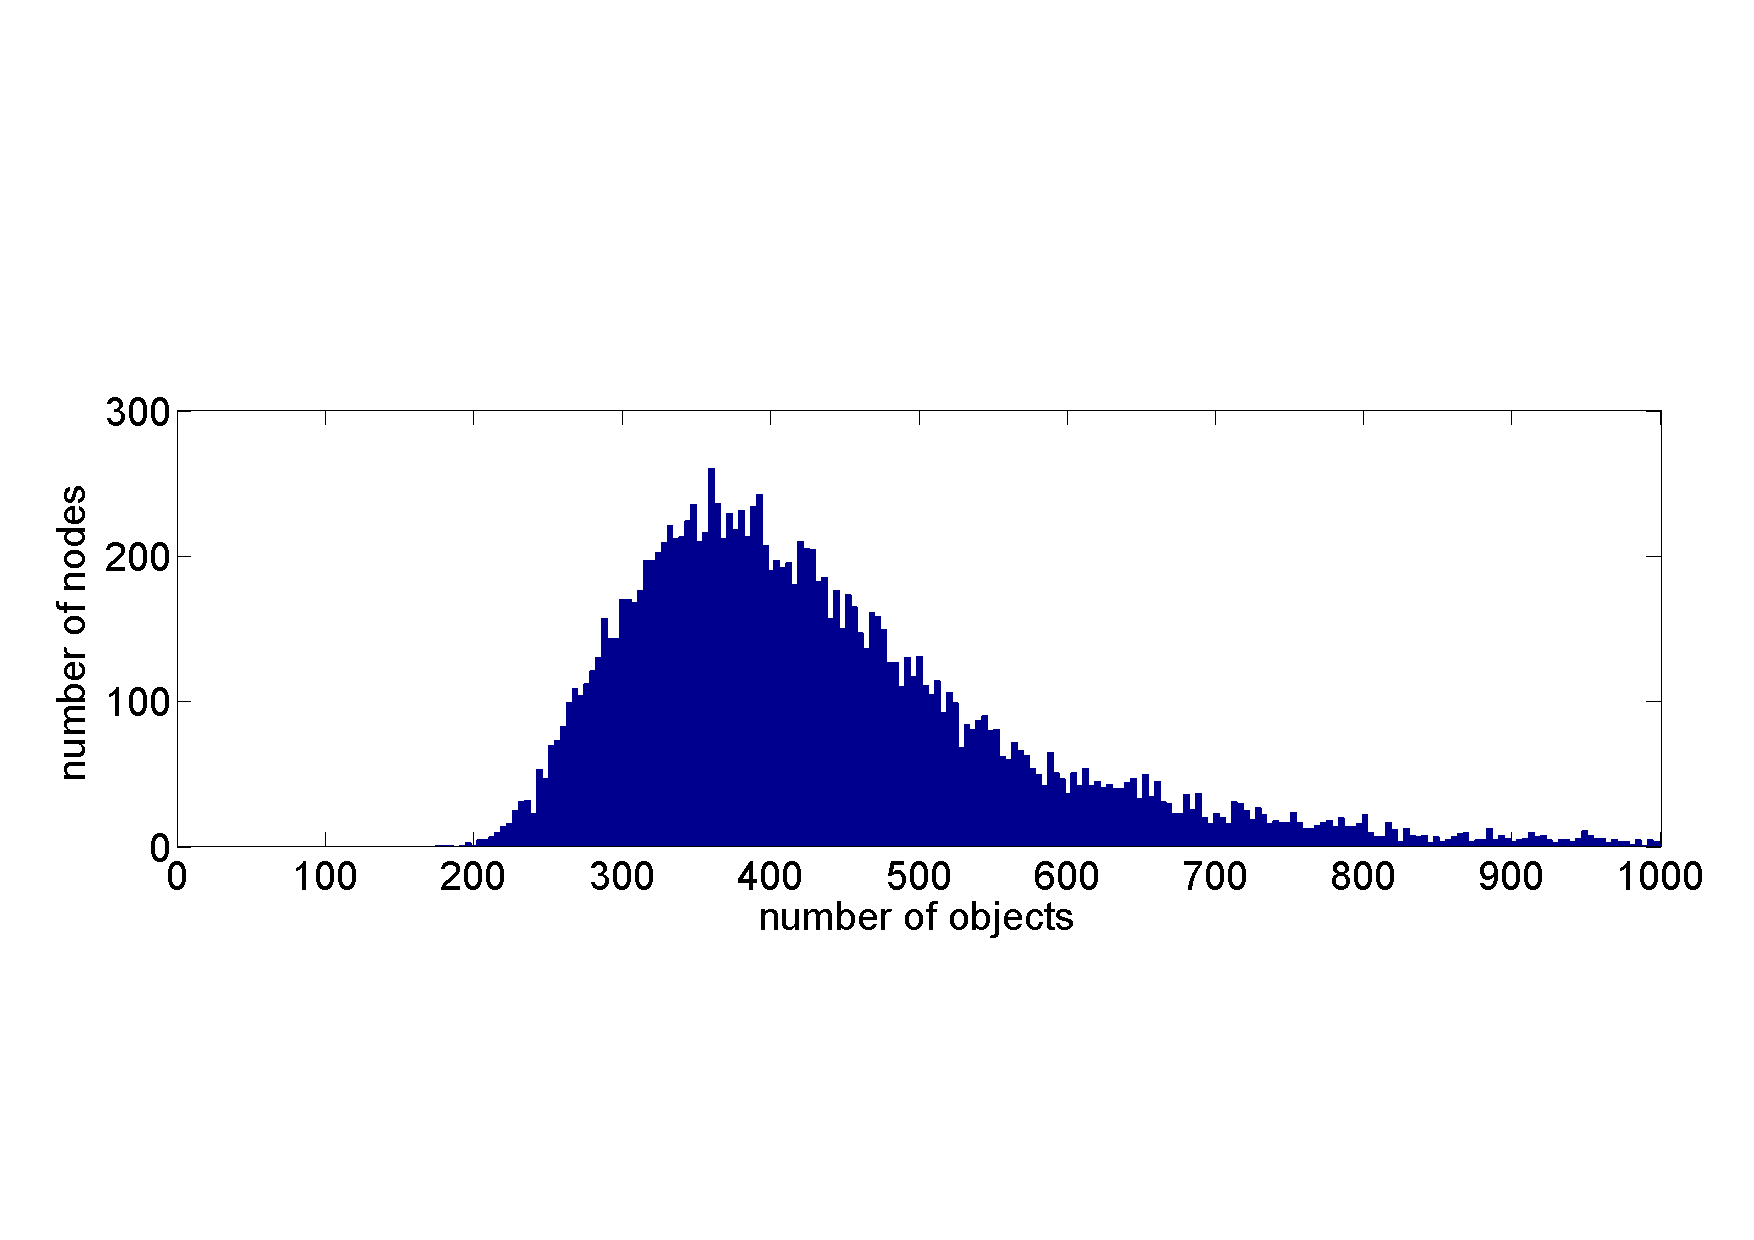
\includegraphics[clip=true, viewport=1.5cm 1.2cm 27cm 19.7cm, width=\columnwidth]{Objects}
 \caption{Combined object number distribution}
 \label{fig_pithos_response}
\end{figure}

Figure \ref{} shows the fairness achieved by mapping file hashes to nodes with the closest IDs. This has the effect of mapping one set of uniform
random numbers onto another set of uniform random numbers, where the two sets are statistically independent. This mapping produces a bernoulli
distribution in the following way:

\begin{figure}[htbp]
 \centering
 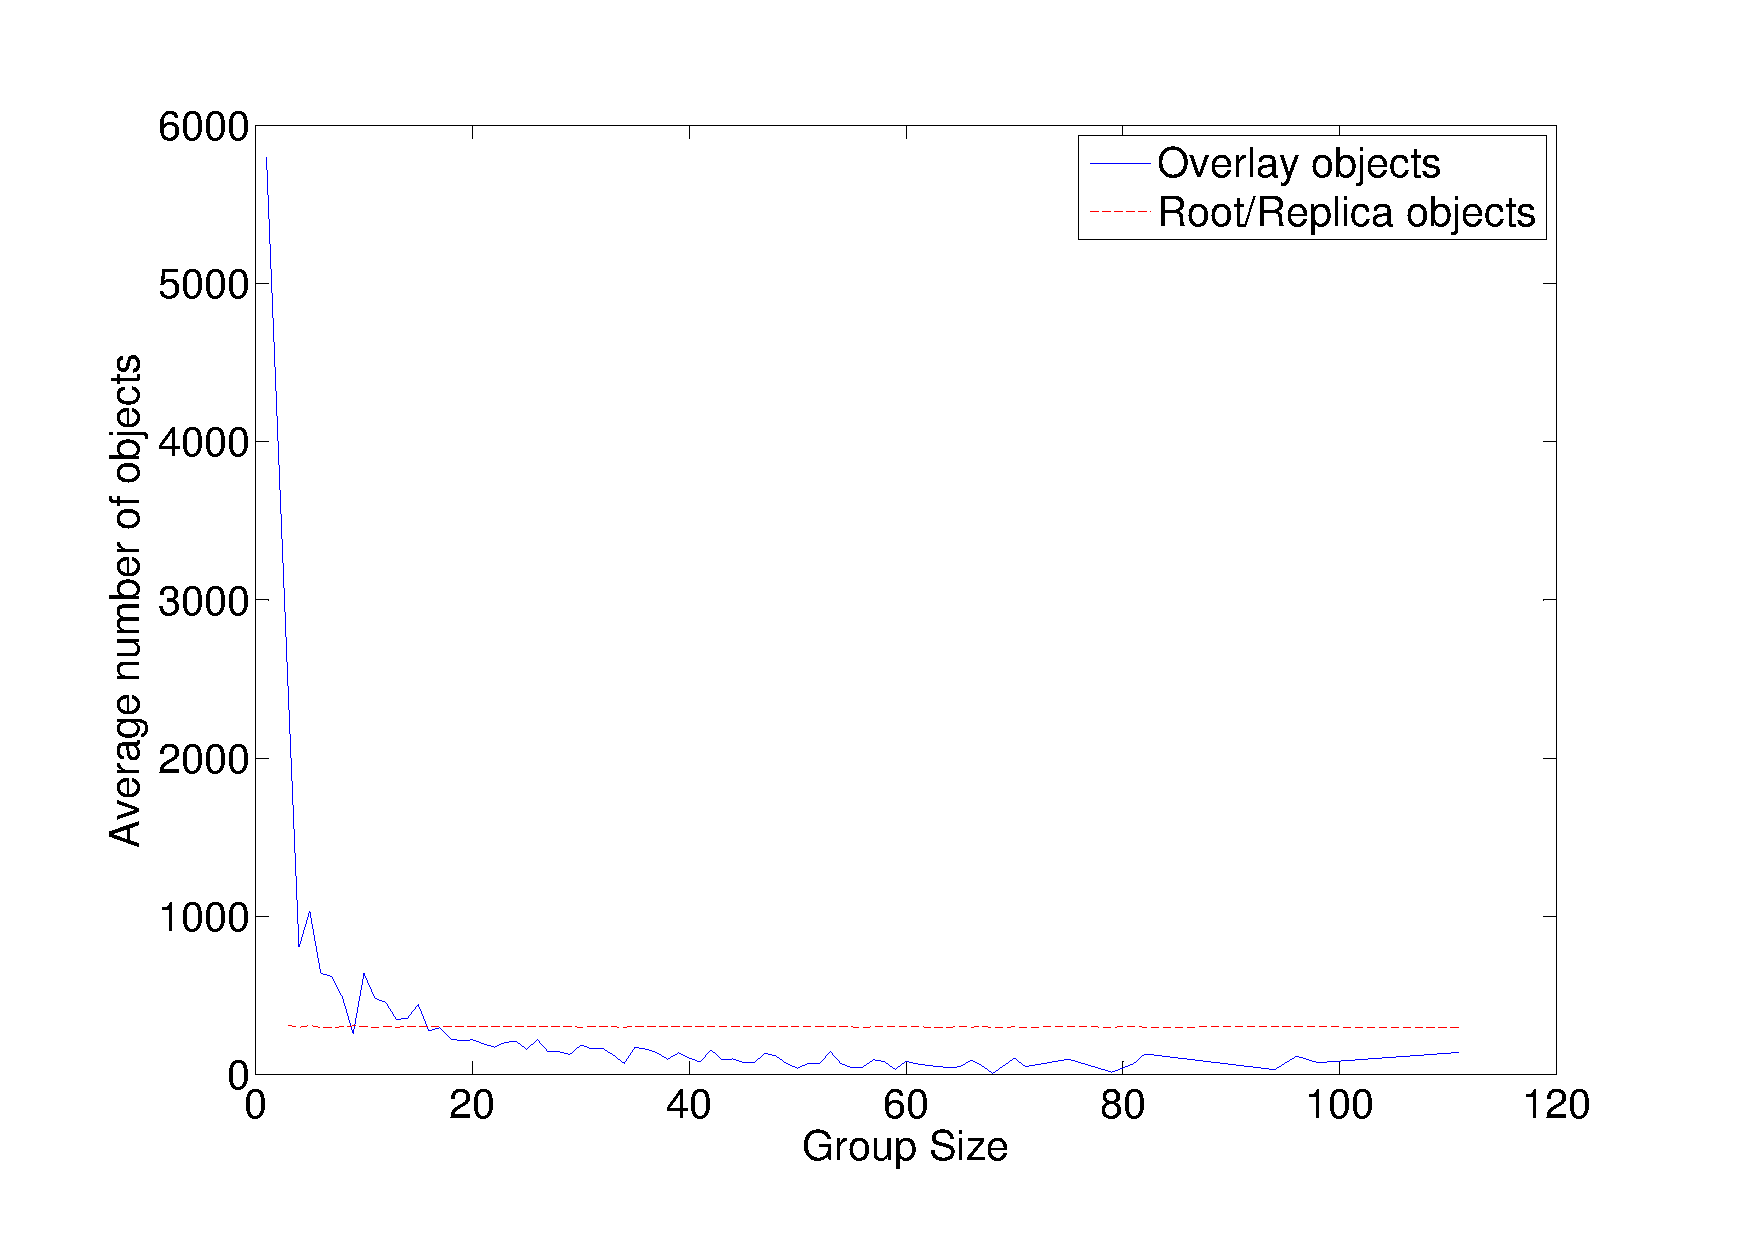
\includegraphics[clip=true, viewport=1.5cm 1cm 27cm 19.5cm, width=\columnwidth]{ObjectsByGroupSize}
 \caption{Average number of overlay objects stored by group size}
 \label{fig_pithos_response}
\end{figure}

\begin{figure}[htbp]
 \centering
 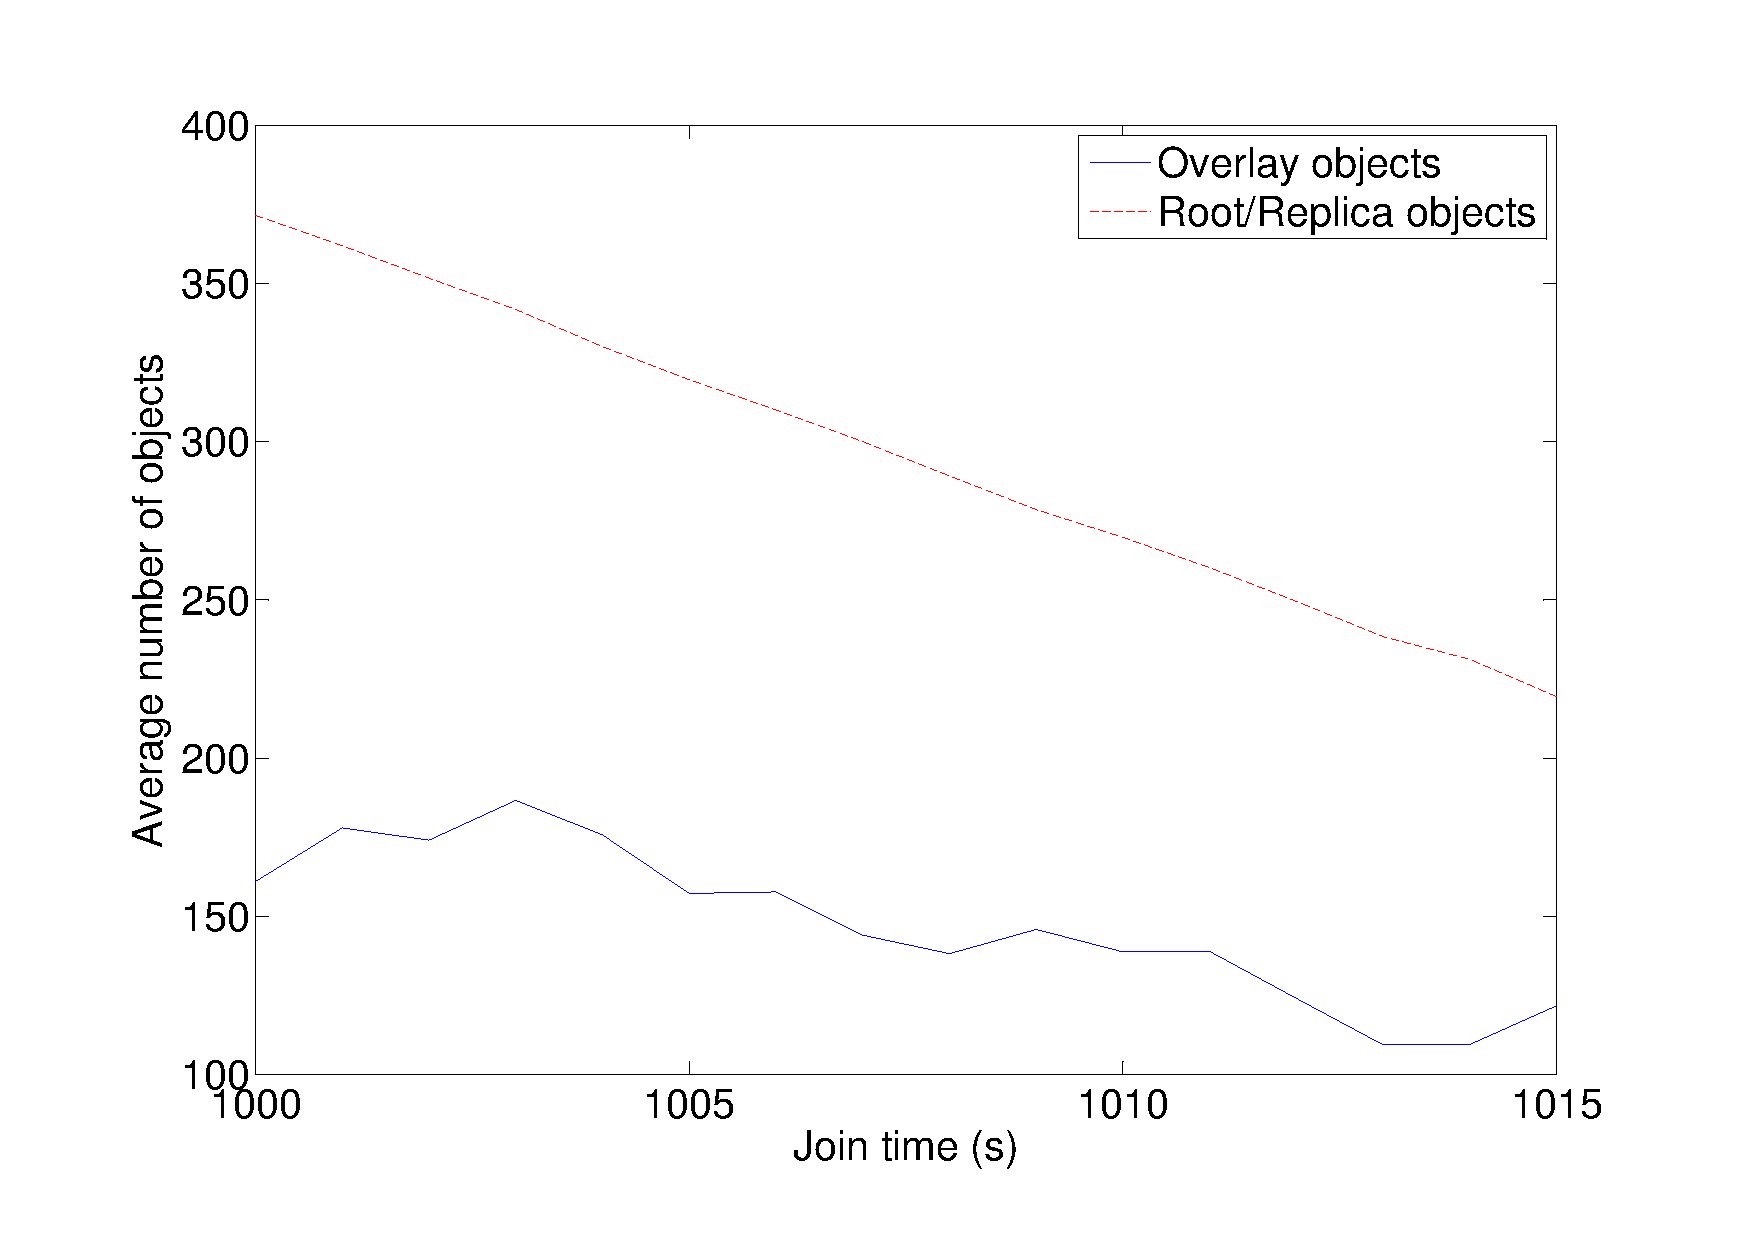
\includegraphics[clip=true, viewport=2cm 1cm 27.5cm 19.5cm, width=\columnwidth]{ObjectsByJoinTime}
 \caption{Average number of overlay objects stored by join time}
 \label{fig_pithos_response}
\end{figure}

%Statistics proof of distribution for constant area and mention that the area is not constant and that adds some jitter to the distribution.
%Note on where the average values come from: 300 and 150 objects per node and 30 nodes per group

\section{Conclusion}
\label{conclusion}

\subsection{Summary}

\subsection{Future work}

%Complete implementation
%Reliability and security
%Driver data

%\newpage
% use section* for acknowledgement
\ifCLASSOPTIONcompsoc
  % The Computer Society usually uses the plural form
  \section*{Acknowledgments}
\else
  % regular IEEE prefers the singular form
  \section*{Acknowledgment}
\fi

The financial assistance of MIH and the National Research Foundation (NRF) towards this research is hereby acknowledged. Opinions expressed and
conclusions arrived at, are those of the author and are not necessarily to be attributed to MIH or the NRF.

%\newpage
%\IEEEtriggeratref{43} %Balance the bibliography
\bibliographystyle{IEEEtran}
\bibliography{../BibTeX/P2P_MMOG}

% that's all folks
\end{document}
